\section{Results} \label{sec:results}
\subsection{Localization precision of the microscope} \label{sec:results_beads}
A set of 100 images of the fluorescent 0.1 \unit{\micro m} beads were acquired for each of the laser wavelengths.
An isolated bead was selected and its intensity profile was fitted in all images with a two-dimensional Gaussian curve. 
The mean and standard variation of the resulting curve provide the $(x,y)$ localisation of the bead and the width of its PSF, as described in \autoref{sec:SMLM}.
An example of the result of the localization, superimposed on one of the images acquired with the 647 nm laser, is depicted in \autoref{fig:beads_inset_zoom}.
%
\begin{figure}[hb]
    \centering
    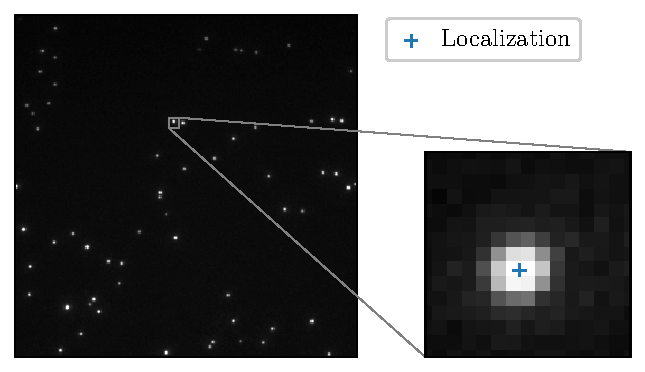
\includegraphics[scale=1]{figures/beads_inset_zoom.pdf}
    \caption{Fluorescent beads imaging using 647 nm laser: whole acquisition  and zoom on selected bead with localised position.}
    \label{fig:beads_inset_zoom}
\end{figure}
%
The distributions of the relative $x$ and $y$ positions obtained from each image are pictured in \autoref{fig:comparison_mu}.
The same was done in \autoref{fig:comparison_sigma} for the uncertainty on the localisation.
%
\begin{figure}[htbp]
    \begin{subfigure}{0.49\textwidth}
        \centering
        {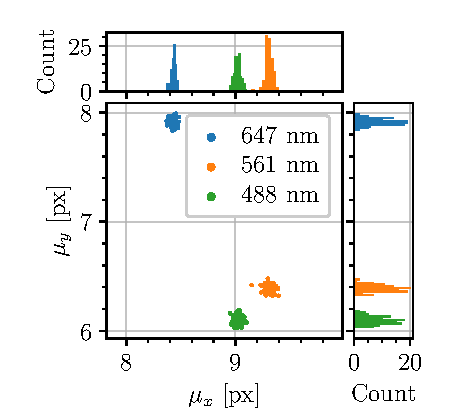
\includegraphics[scale=1]{figures/comparison_mu.pdf}}
        \caption{}
        \label{fig:comparison_mu}
    \end{subfigure}
    \begin{subfigure}{0.49\textwidth}
        \centering
        {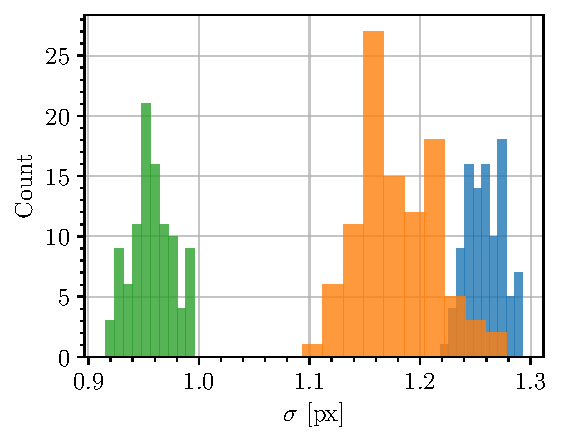
\includegraphics[scale=1]{figures/comparison_sigma.pdf}}
        \caption{}
        \label{fig:comparison_sigma}
    \end{subfigure}
    \caption{Comparison of (a) localisation position and (b) uncertainty distributions for the three different laser wavelengths. One pixel corresponds to $108$ nm.}
    \label{fig:comparison_wavelengths}
\end{figure}
%
The figures allow for a couple of immediate observations:
the localisations carried out using each of the three different wavelengths cluster around three different points, though the sample wasn't moved between acquisitions.
This is due to a drifting of the fluorescent beads in the focal plane (see \autoref{fig:beads_drifting}), the three acquisitions being separated by intervals of time much longer than the time scale of a single acquisition (all the data was acquired over the course of \mbox{3 hours}).
%
\begin{figure}
    \centering
    \begin{subfigure}{0.32\textwidth}
        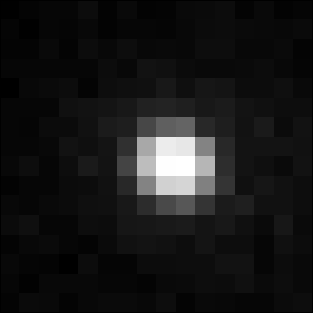
\includegraphics[width=\textwidth]{figures/beads_drifting_647nm.pdf}
        \caption{}
        \label{fig:beads_drifting_647nm}
    \end{subfigure}
    \begin{subfigure}{0.32\textwidth}
        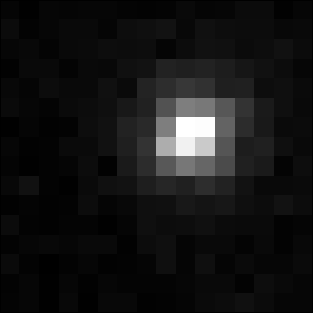
\includegraphics[width=\textwidth]{figures/beads_drifting_561nm.pdf}
        \caption{}
        \label{fig:beads_drifting_561nm}
    \end{subfigure}
    \begin{subfigure}{0.32\textwidth}
        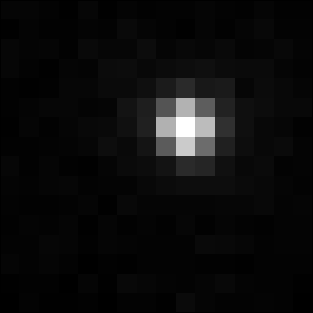
\includegraphics[width=\textwidth]{figures/beads_drifting_488nm.pdf}
        \caption{}
        \label{fig:beads_drifting_488nm}
    \end{subfigure}
    \caption{Drifting between acquisitions of the studied fluorescent bead during the consecutive acquisitions with the (a) 647 nm (b) 561 nm and (c) 488 nm lasers.}
    \label{fig:beads_drifting}
\end{figure}
%
Moreover, the uncertainties on the localisation for the different wavelengths appear to center around different points, the 488 nm laser resulting the most precise of the three.
These values were compared with those expected from \autoref{eq:PSF_width_gaussian} for the PSF width associated to each mesure.
As shown in \autoref{fig:comparison_PSF}, while increasing with $\lambda$ as predicted,
the observed PSF width is higher than the one expected.
\begin{figure}[htbp]
    \centering
    \vspace{-0.5cm}
    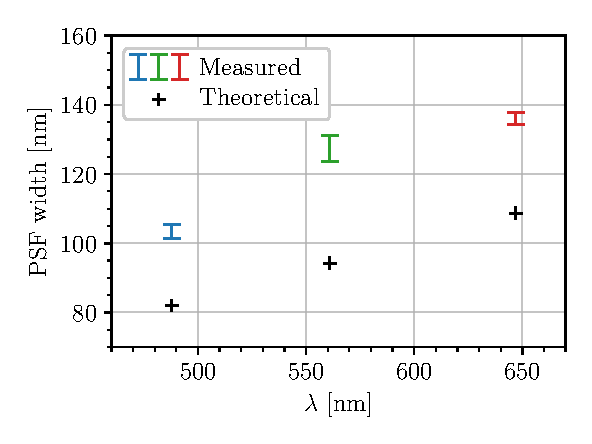
\includegraphics[scale=1]{figures/comparison_PSF.pdf}
    \caption{Measured Gaussian PSF width compared with theoretical values, for multiple laser wavelengths.}
    \label{fig:comparison_PSF}
\end{figure}


\subsection{STORM imaging of microtubules} \label{sec:results_microtubules}
A set of three STORM images of microtubules in COS7 cells are presented in \autoref{fig:microtubules_images}.
%
\begin{figure}
    \begin{subfigure}{0.32\textwidth}
        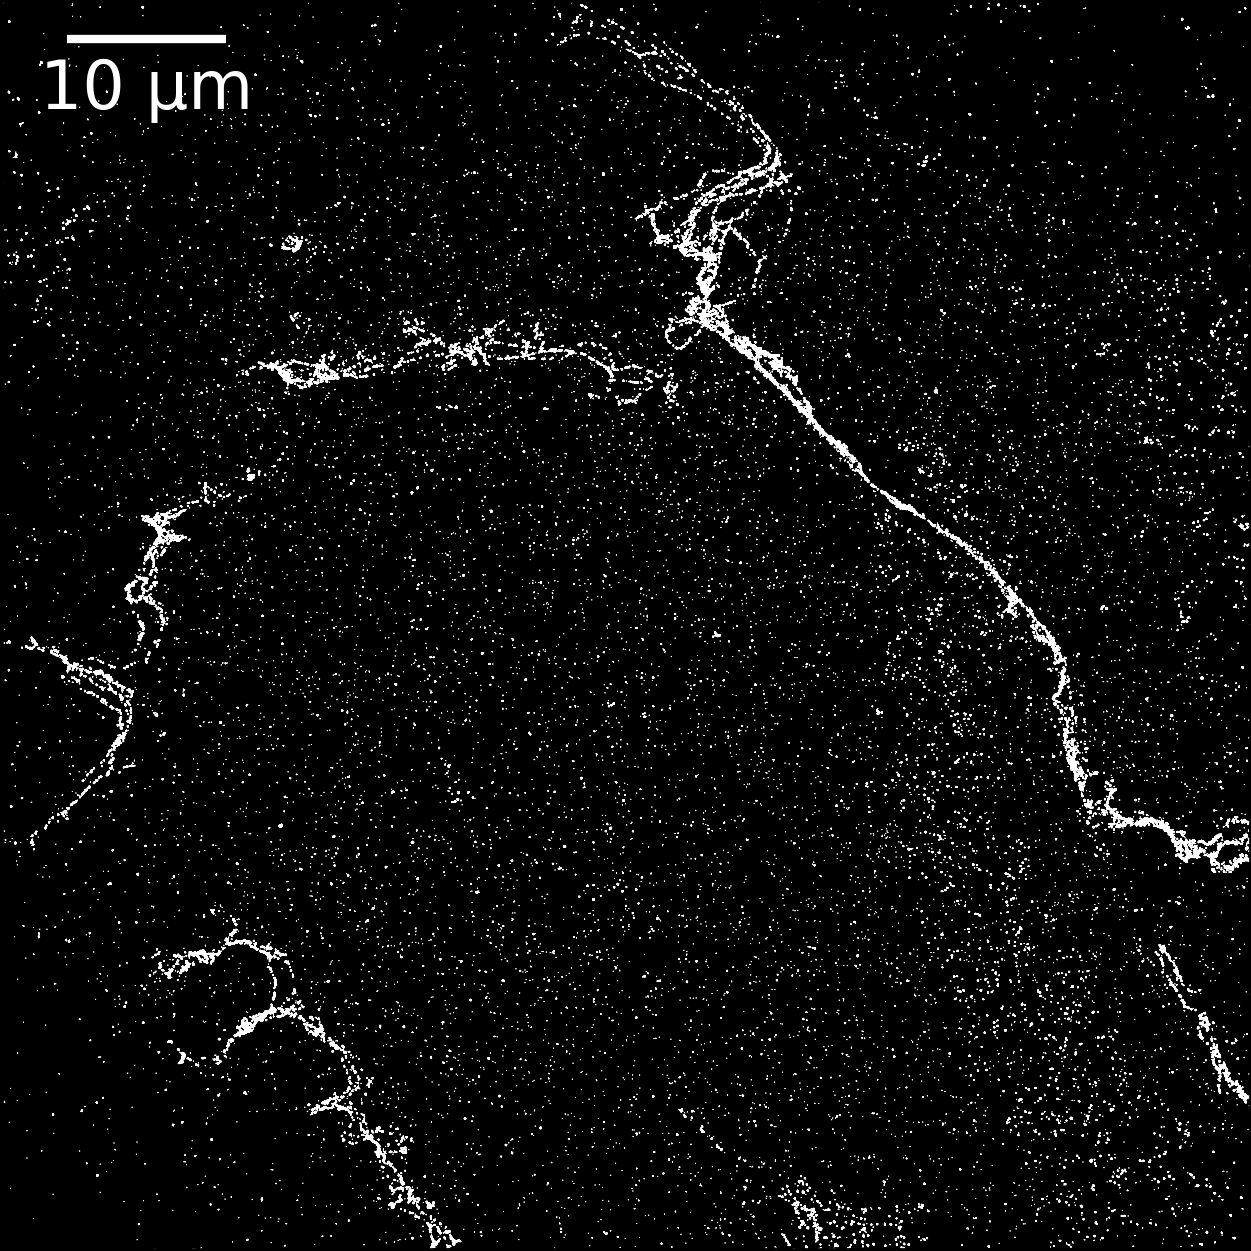
\includegraphics[width=\textwidth]{figures/microtubules_image1.png}
        \caption{}
        \label{fig:microtubules_image1}
    \end{subfigure}
    \begin{subfigure}{0.32\textwidth}
        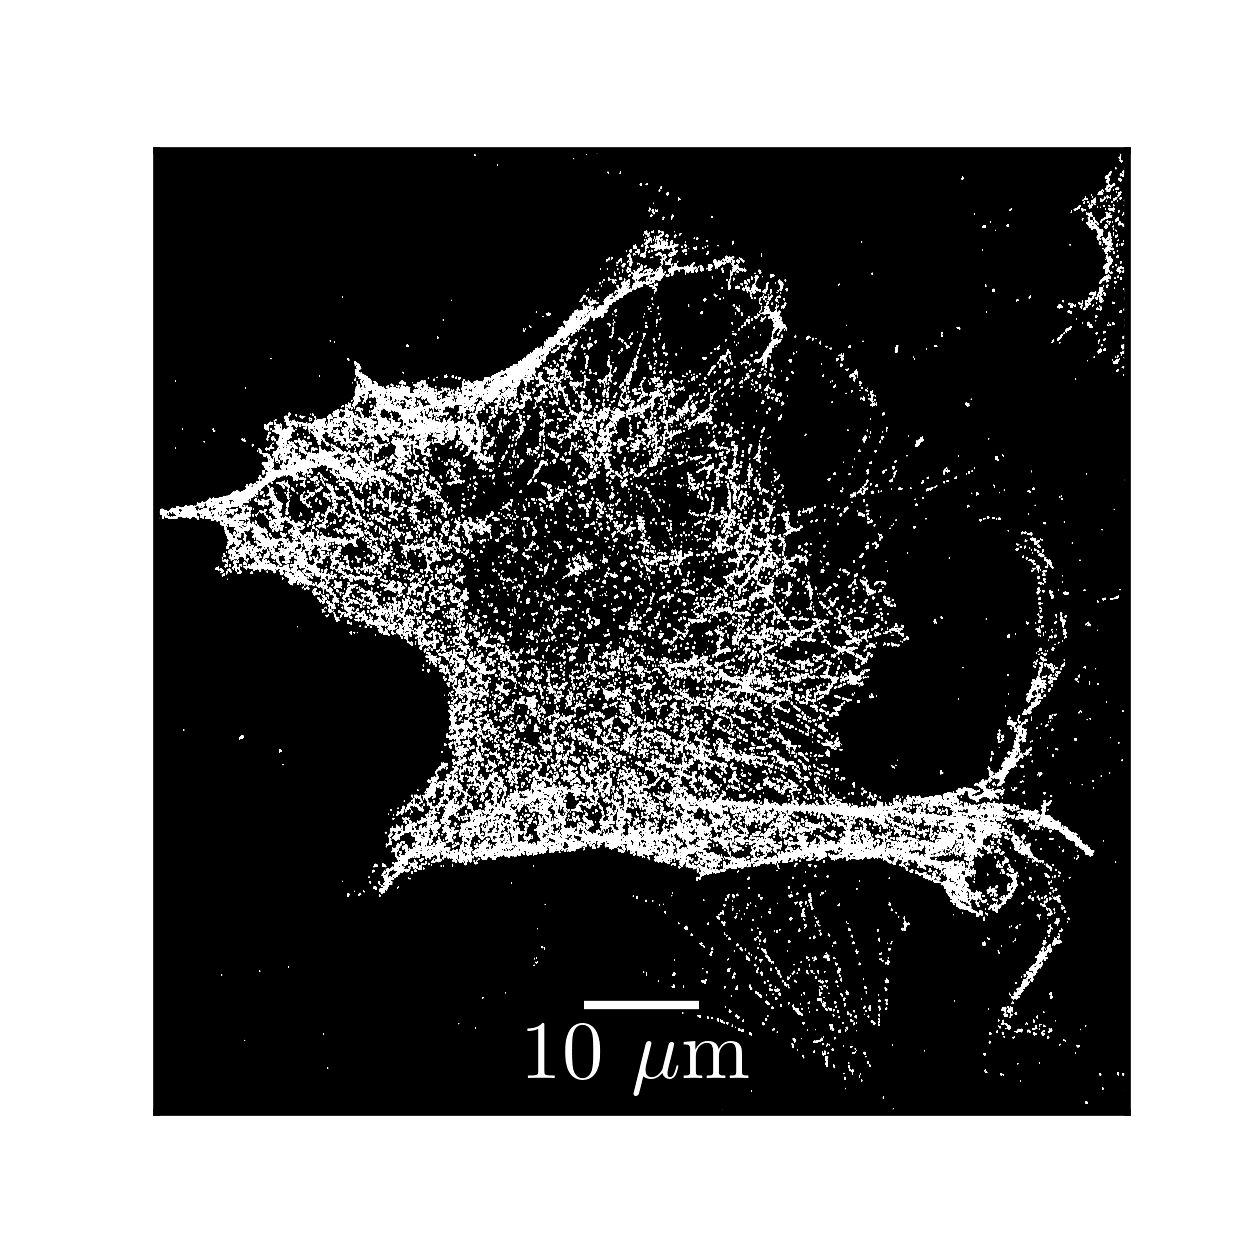
\includegraphics[width=\textwidth]{figures/microtubules_image4.png}
        \caption{}
        \label{fig:microtubules_image4}
    \end{subfigure}
    \begin{subfigure}{0.32\textwidth}
        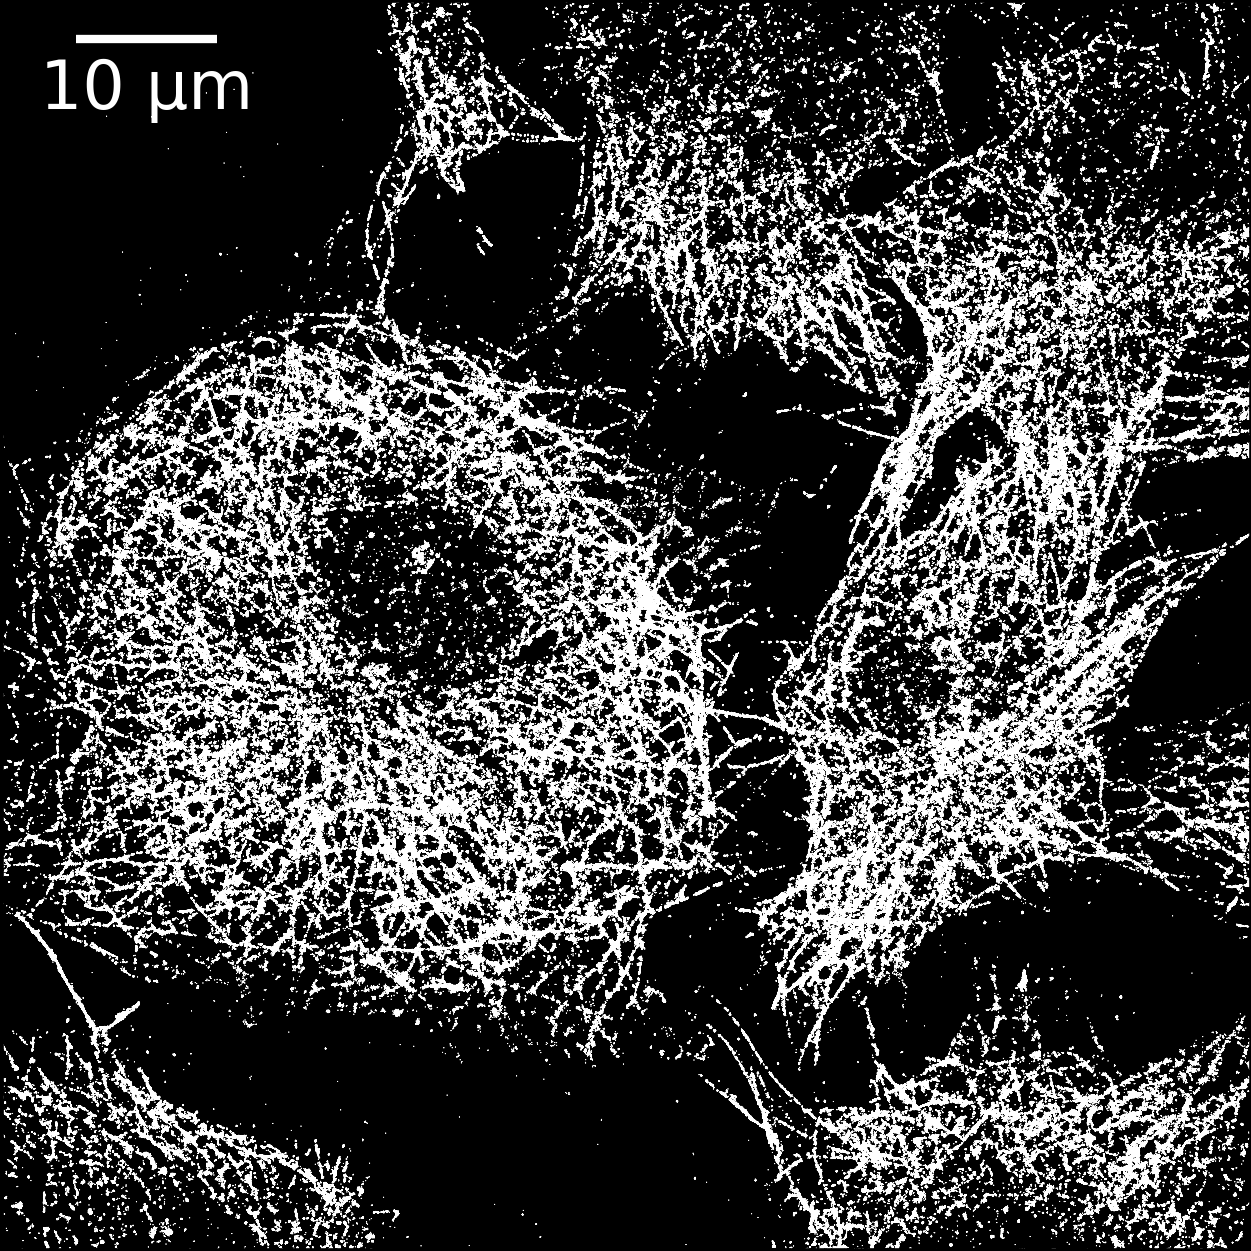
\includegraphics[width=\textwidth]{figures/microtubules_image6.png}
        \caption{}
        \label{fig:microtubules_image6}
    \end{subfigure}
    \caption{STORM images of microtubules in COS7 cells.}
    \label{fig:microtubules_images}
\end{figure}
%
\autoref{fig:microtubules_image1} shows an isolated microtubule, while in \autoref{fig:microtubules_image4} and \autoref{fig:microtubules_image6} it is possible to distinguish the overall structure of the cytoskeleton, composed of a large number of microtubules, and the nuclei of the cells, recognisable as the circular areas of lower localisation density.
An analysis of the intensity profile along the cross section of the microtubule strand in \autoref{fig:microtubules_image1} showed the presence of two distinct peaks, separated by a distance of $(210 \pm 5)$ nm.
The portion of filament studied and the resulting intensity profile are depicted in \autoref{fig:microtubules_width}.
%
\begin{figure}[htbp]
    \begin{subfigure}[b]{0.49\textwidth}    % trim left bottom right top
        \centering
        \raisebox{0.5cm}{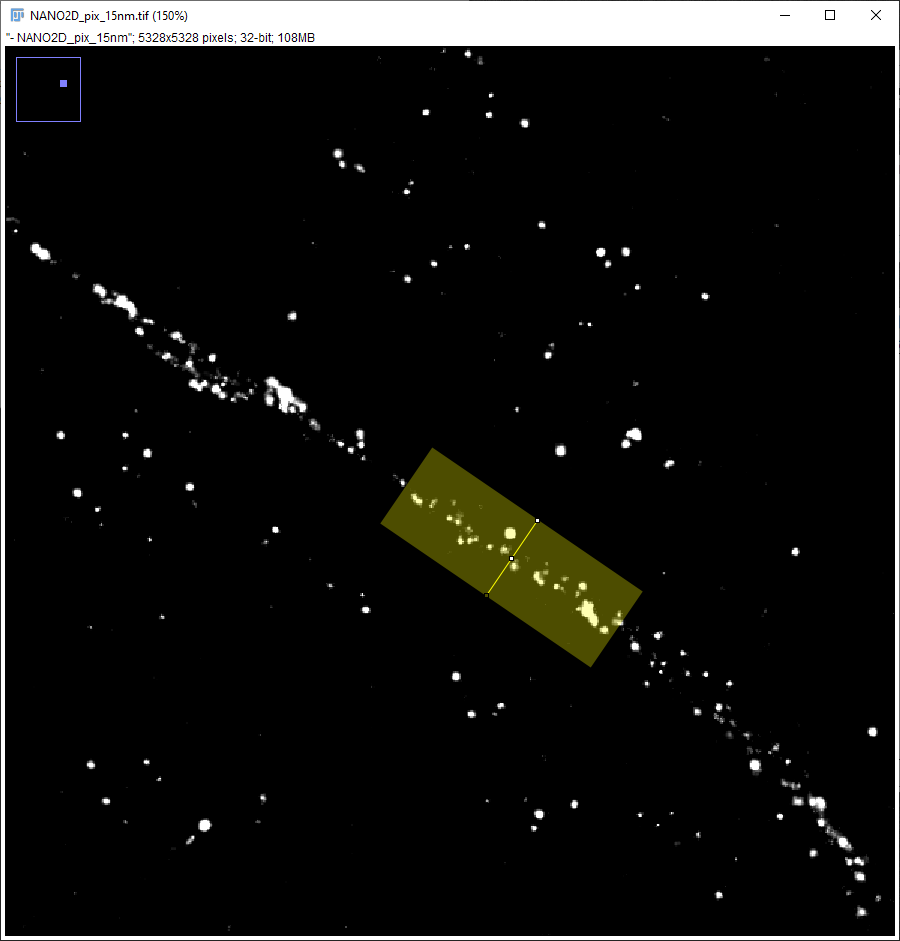
\includegraphics[width=0.9\textwidth, trim={1cm 1.5cm 1cm 5cm}, clip]{figures/microtubules_width_acquisition.PNG}}
        \caption{}
        \label{fig:microtubules_width_acquisition}
    \end{subfigure}
    \begin{subfigure}[b]{0.49\textwidth}
        \centering
        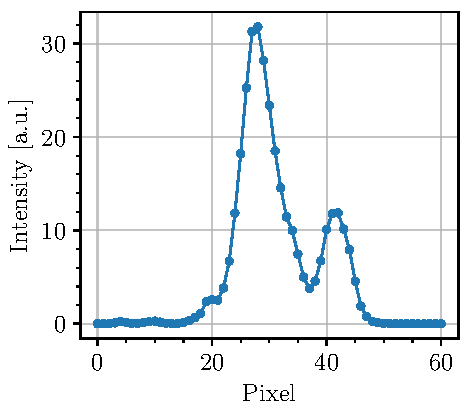
\includegraphics[scale=1]{figures/microtubules_width.pdf}
        \caption{}
        \label{fig:microtubules_width_analysis}
    \end{subfigure}
    \caption{Intensity profile along a microtubule strand: (a) screen capture of the profile acquisition using the \software{Fiji} processing package, (b) the intensity profile averaged over the portion of length considered.}
    \label{fig:microtubules_width}
\end{figure}


\subsection{STORM imaging of mitochondria} \label{sec:results_mitochondria}
STORM images of the mitochondrial network in COS7 cells (see \autoref{fig:mitochondria_images}) were able to distinguish individual mitochondria surrounding the nucleus, for which the cross section could then be determined.
In the measured set of 18 mitochondria, the cross sections ranged from $(0.8 \pm 0.1)$ \unit{\micro\meter\squared} to $(4.3 \pm 0.3)$ \unit{\micro\meter\squared}, with an average of $(2.21 \pm 0.06)$ \unit{\micro\meter\squared}. The complete set of measurements are shown in \autoref{tab:mitochondria_cross_sections}.
%
\begin{figure}
    \centering
    \begin{subfigure}{0.49\textwidth}
        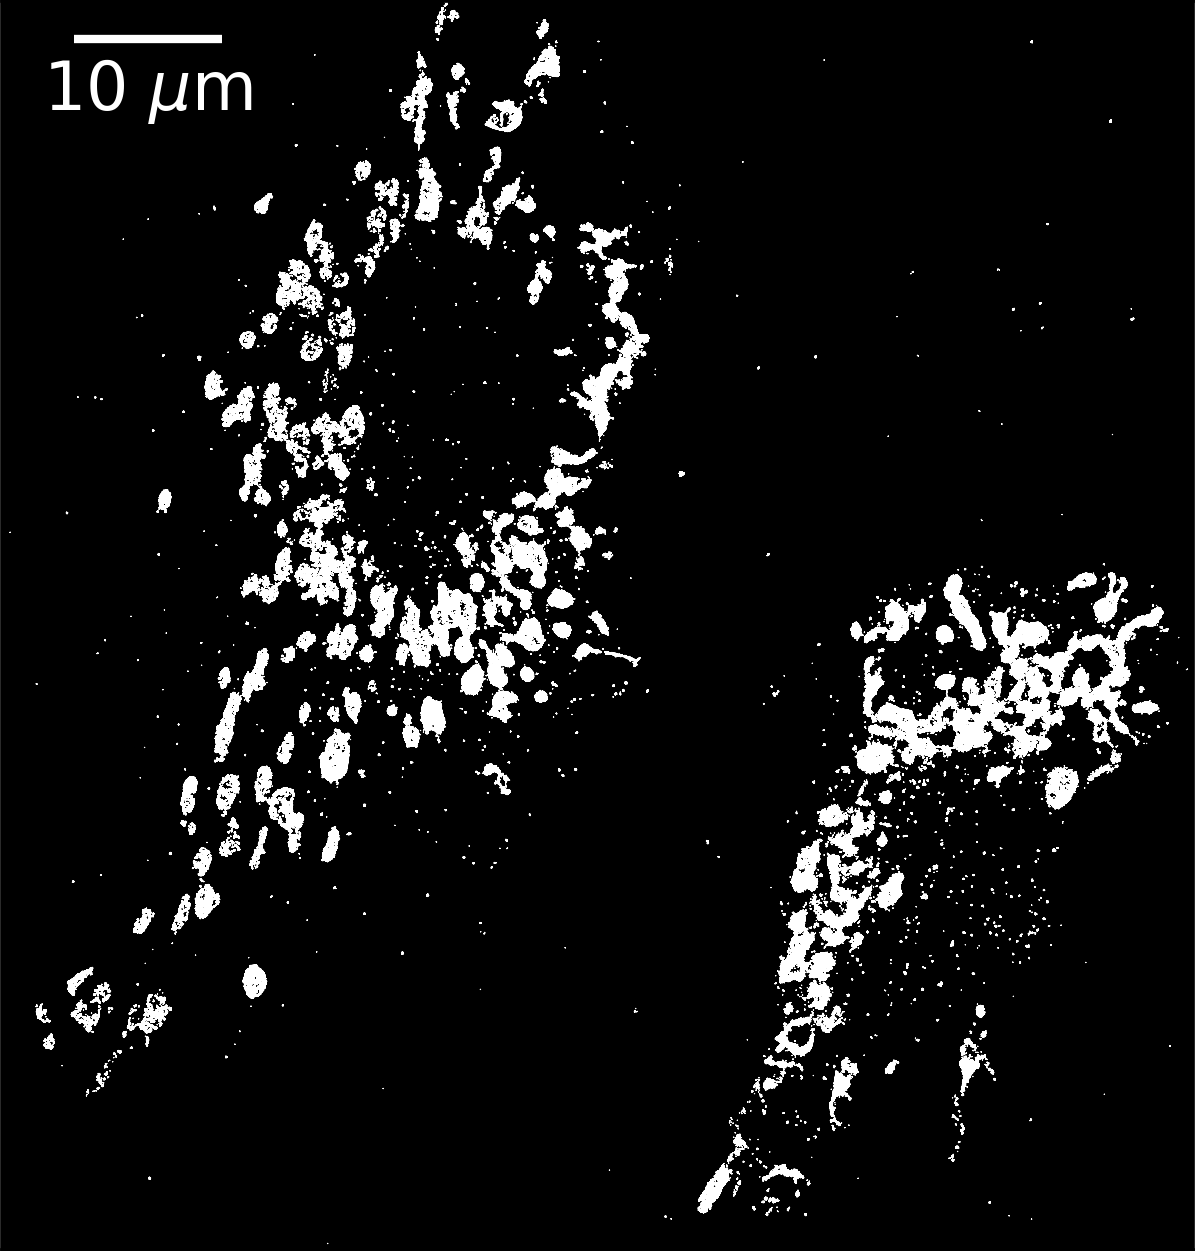
\includegraphics[width=\textwidth]{figures/mitochondria_image4.png}
        \caption{}
        \label{fig:mitochondria_image4}
    \end{subfigure}
    \begin{subfigure}{0.49\textwidth}
        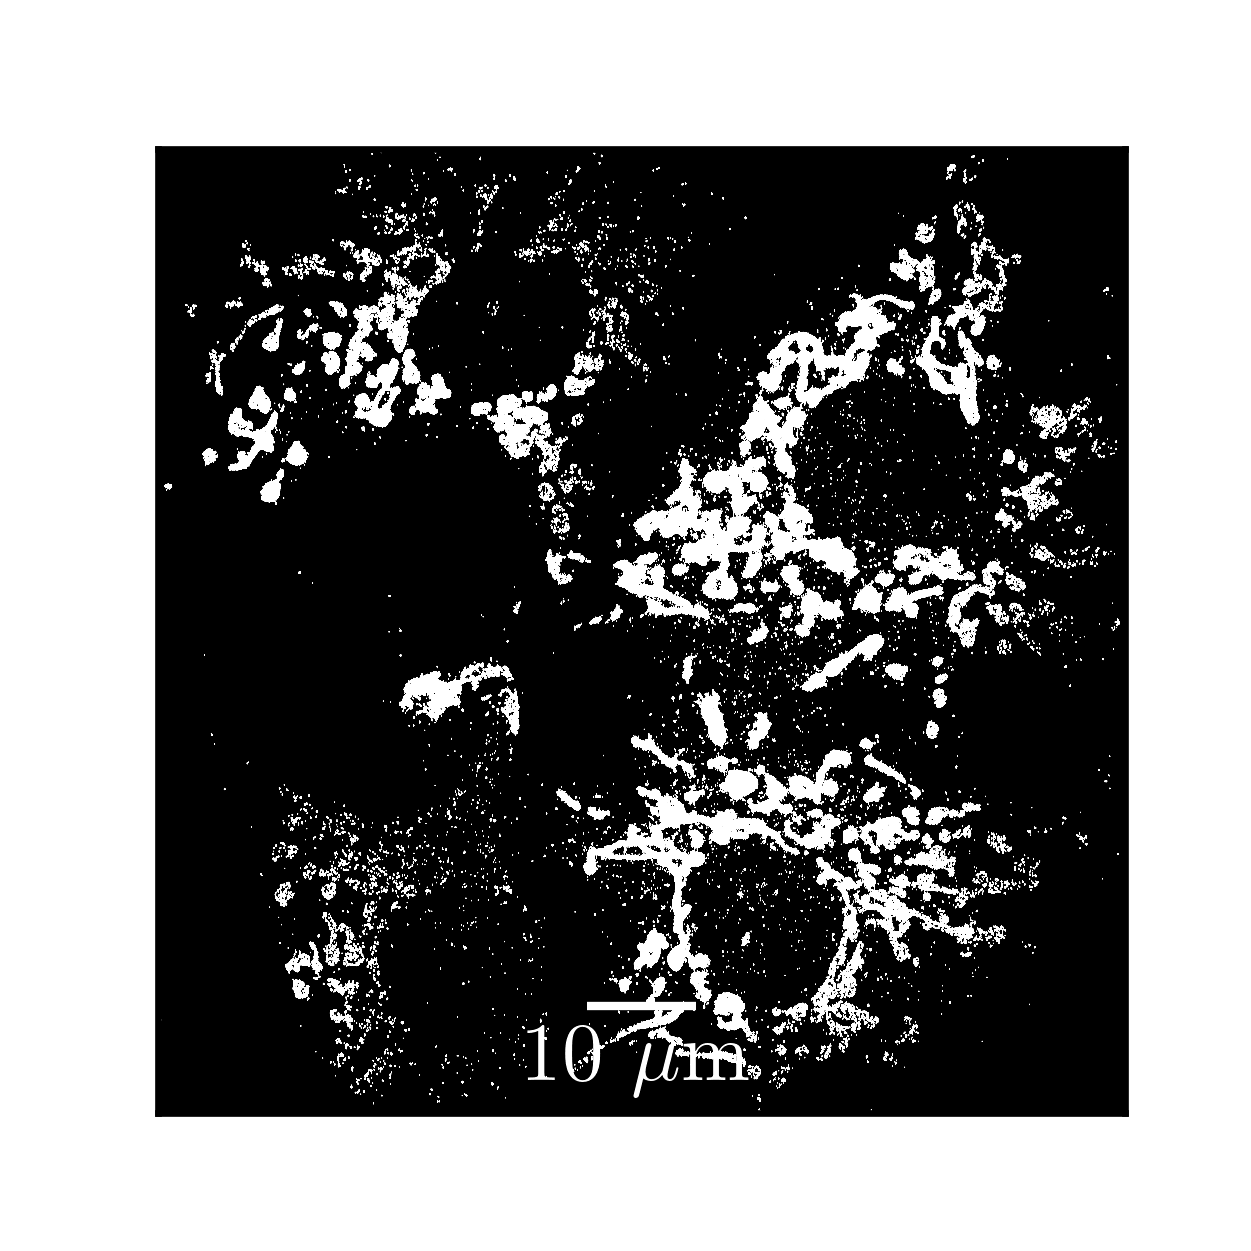
\includegraphics[width=\textwidth]{figures/mitochondria_image11.png}
        \caption{}
        \label{fig:mitochondria_image11}
    \end{subfigure}
    \caption{STORM images of mitochondrial structures in COS7 cells.}
    \label{fig:mitochondria_images}
\end{figure}

\begin{table}
    \centering
    \begin{tabular}{c|c|c|c|c|c}
        \multicolumn{6}{c}{Cross sections [\si{\micro\meter\squared}]} \\
        \hline\hline
		$\left(0.8 \pm 0.1\right)$ & $\left(1.0 \pm 0.1\right)$ & $\left(1.2 \pm 0.2\right)$ & $\left(1.5 \pm 0.2\right)$ & $\left(1.5 \pm 0.2\right)$ & $\left(1.6 \pm 0.2\right)$ \\
		$\left(1.6 \pm 0.2\right)$ & $\left(1.7 \pm 0.2\right)$ & $\left(1.9 \pm 0.2\right)$ & $\left(2.2 \pm 0.2\right)$ & $\left(2.2 \pm 0.2\right)$ & $\left(2.3 \pm 0.2\right)$ \\
		$\left(2.4 \pm 0.3\right)$ & $\left(3.1 \pm 0.3\right)$ & $\left(3.2 \pm 0.3\right)$ & $\left(3.7 \pm 0.4\right)$ & $\left(3.7 \pm 0.3\right)$ & $\left(4.3 \pm 0.3\right)$
    \end{tabular}
    \caption{Measured cross sections of captured mitochondria, sorted in ascending order}
    \label{tab:mitochondria_cross_sections}
\end{table}


\subsection{STORM imaging of clathrin} \label{sec:results_clathrin}
Several STORM images of the labeled clathrin in COS7 cells were acquired, such as the ones presented in \autoref{fig:clathrin_images}.
It is possible in these images to recognise the outer boundaries of the cytoplasm (the circular areas of low localisation density, larger than the nuclei observed in \autoref{sec:results_microtubules} and \autoref{sec:results_mitochondria}), enclosed by the cell membrane on which the clathrin is found.
%
\begin{figure}
    \centering
    \begin{subfigure}{0.49\textwidth}
        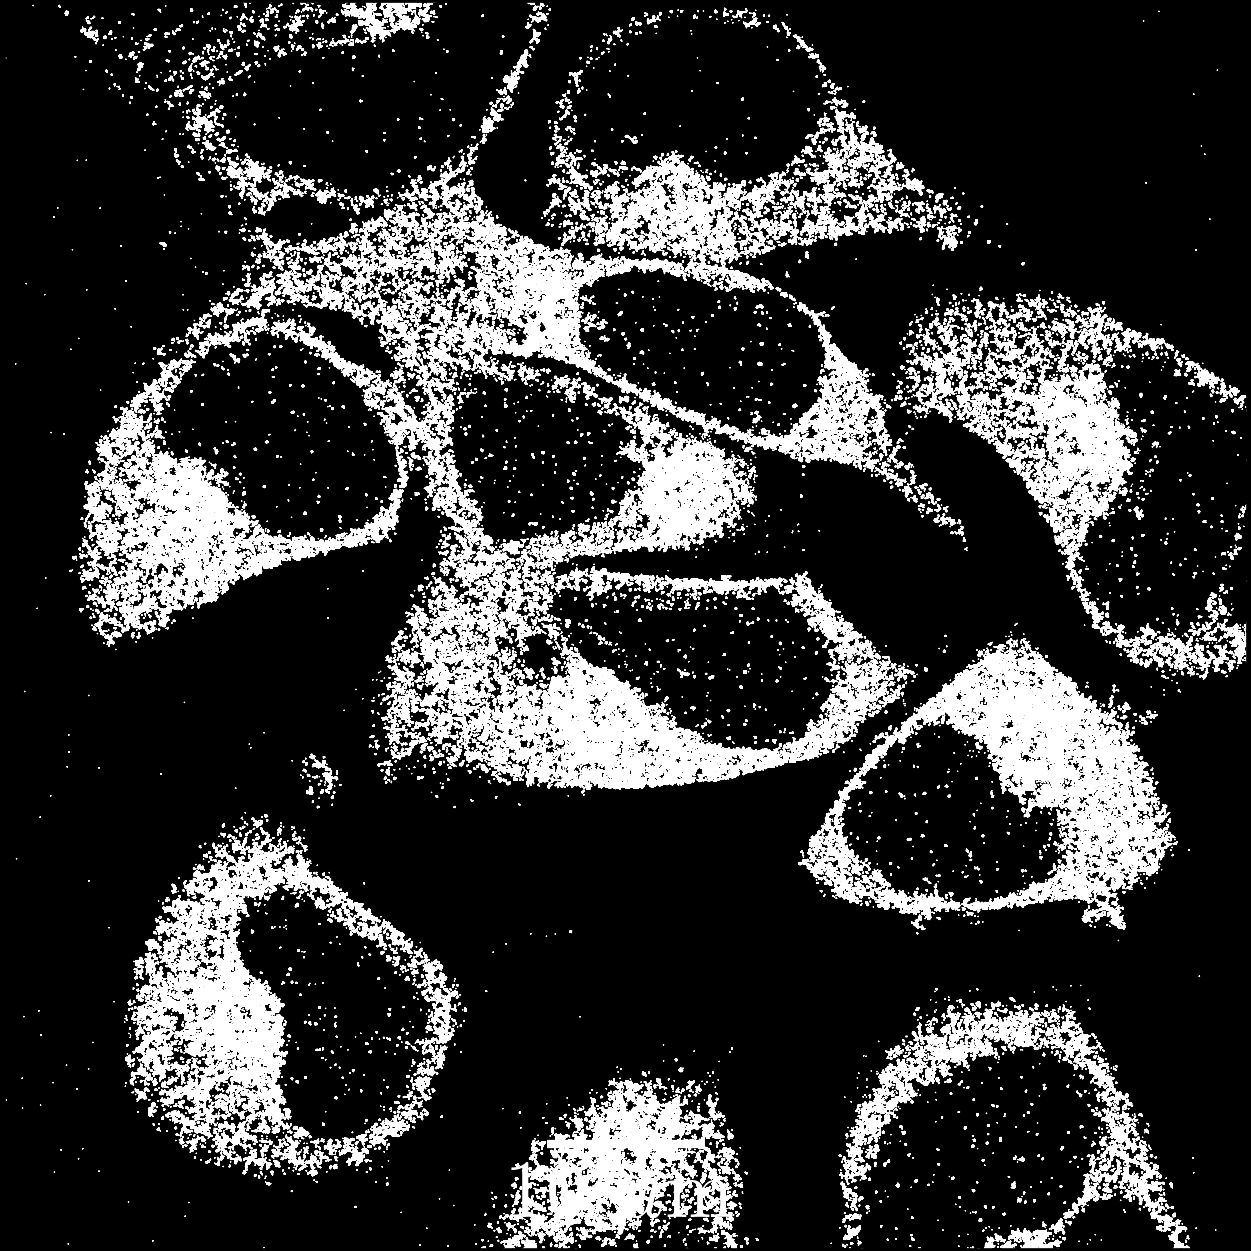
\includegraphics[width=\textwidth]{figures/clathrin_image11.png}
        \caption{}
        \label{fig:clathrin_image1}
    \end{subfigure}
    \begin{subfigure}{0.49\textwidth}
        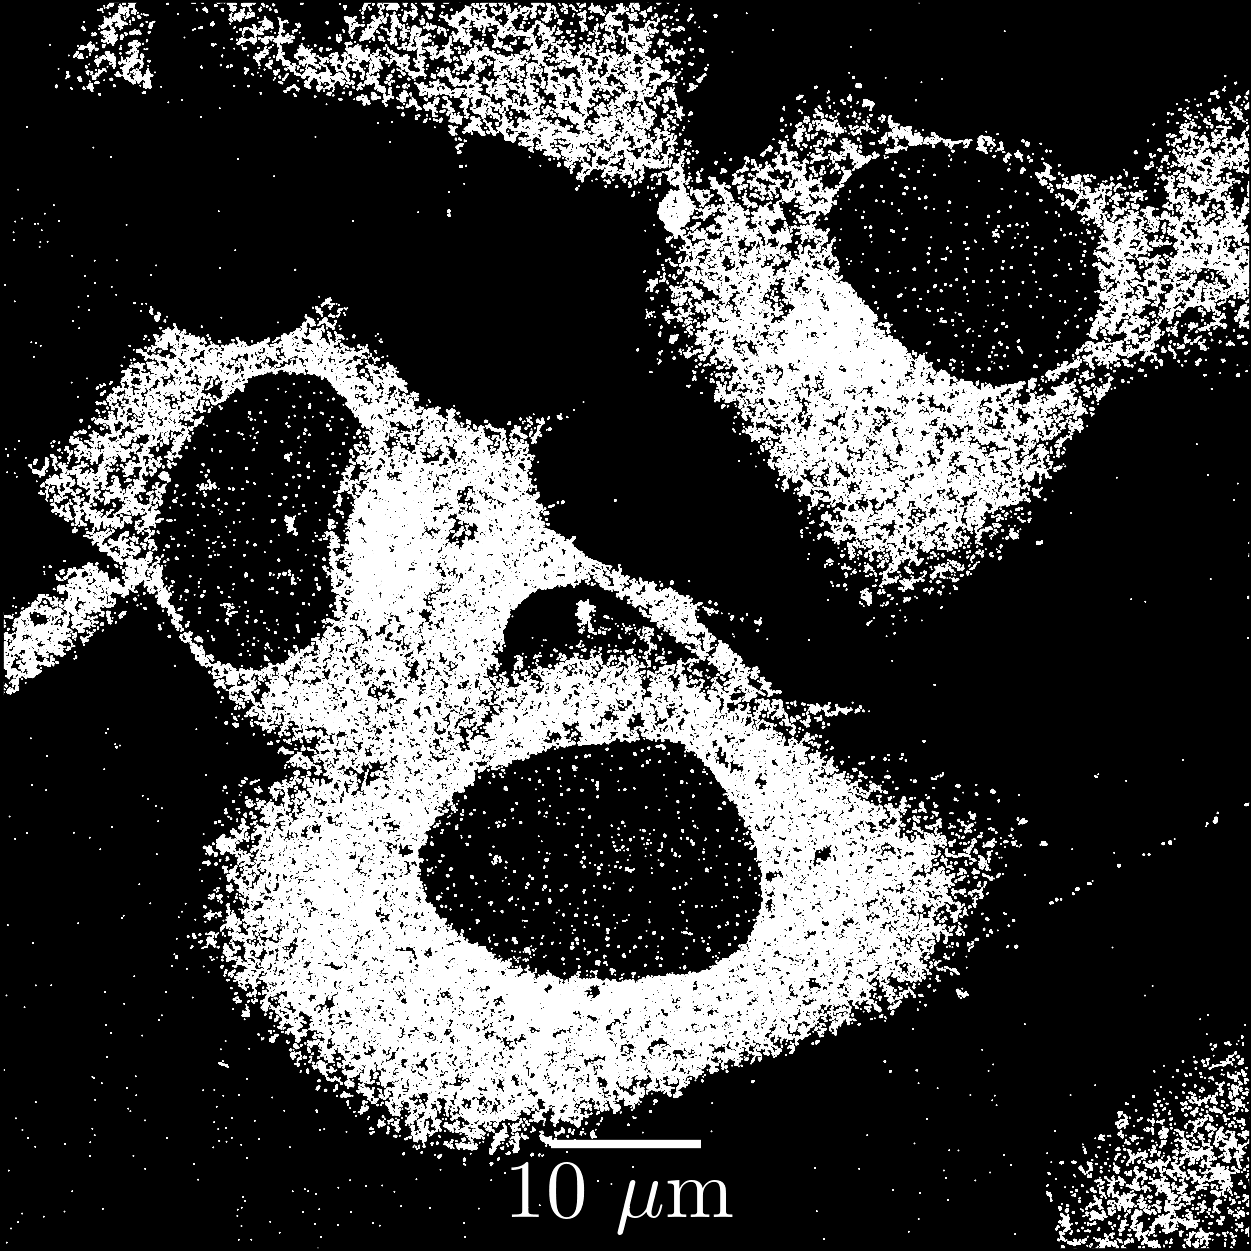
\includegraphics[width=\textwidth]{figures/clathrin_image2.png}
        \caption{}
        \label{fig:clathrin_image6}
    \end{subfigure}
    \caption{STORM imaging of labeled clathrin in COS7 cells.}
    \label{fig:clathrin_images}
\end{figure}

The Annex contains additional STORM images of both mitochondria and clathrin acquired during the experiments (see \autoref{fig:extra_mitochondria_images} and \autoref{fig:extra_clathrin_images}).